\newpage
\section{Signifikanz der Features}
Die Signifikanz der Features wird über die Permutationswichtigkeit bestimmt.
Die Permutationswichtigkeit ist der Fehler, der durch das permutieren eines Features in der Testmenge entsteht, im Vergleich zu der ursprünglichen Testmenge.
Je größer der Fehler, desto wichtiger das Feature.
\newline
\newline
Abbildungen \ref{fig:feature_significance_dt} und \ref{fig:feature_significance_knn} zeigen die Permutationswichtigkeit eines Entscheidungswaldes und FFNN.
Die Features sind abgekürzt in der Grafik: \textit{acc} steht für die Features aus den Accelerometer, \textit{light} für den Lichtsensor, \textit{ap} für den WLAN-Zugangspunkt,
\textit{temperature} für den Temperatursensor, \textit{heading} für den Magnetfeldsensor, \textit{volume} für den Geräuschsensor, \textit{ang} für das Gyroskop.
Die Permutationswichtigkeit von einzelnen Entscheidungswäldern bzw. FFNNs unterscheidet sich nicht stark.
Beide ML-Modelle weisen den vorherigen Standorten eine hohe Signifikanz zu.
Die Klassifizierunggenauigkeiten in Tabelle \ref{tab:predictions_by_acc_pic_cont} bestätigen diese Abhängigkeit.
Demnach ist die Wahrscheinlichkeit sehr gering, dass der Standort korrekt klassifiziert wird, wenn der vorherige Standort inkorrekt war.
\begin{figure}[h!]
    \centering
    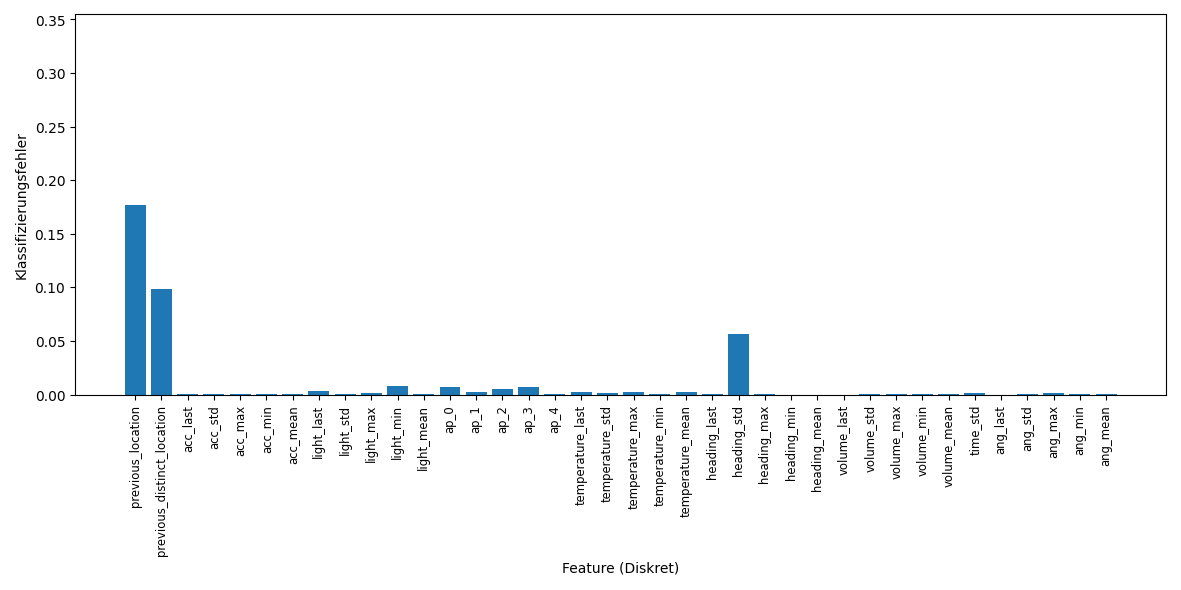
\includegraphics[width=\linewidth]{images/evaluation_feature_importance_dt_pi.png}
    \caption{Permutationswichtigkeit der Features eines Entscheidungswaldes.}
    \label{fig:feature_significance_dt}
\end{figure}
\begin{figure}[h!]
    \centering
    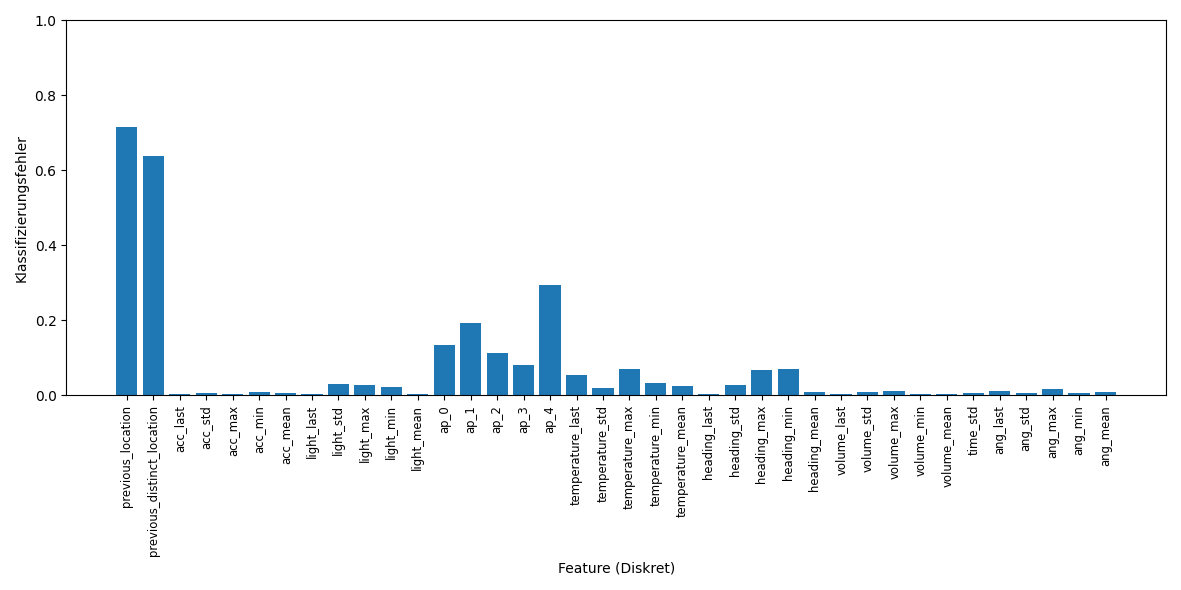
\includegraphics[width=\linewidth]{images/evaluation_feature_importance_knn_pi.png}
    \caption{Permutationswichtigkeit der Features eines FFNN.}
    \label{fig:feature_significance_knn}
\end{figure}
\newline
\newline
Für die Entscheidungswälder sind alle Features, bis auf die vorherige Position und die Standardabweichung von der Ausrichtung zum Magnetfeld unwichtig.
Die FFNNs hingegen bedienen sich außerdem Features von dem Temperatursensor, dem Lichtsensor und vor allem der Detektierung von WLAN-Zugangspunkten.
Allerdings sind FFNNs deutlich abhängiger von dem vorherigen Standort als Entscheidungswälder.
\newline
\newline
Durch diese Abhängigkeit ist keine hohe Robustheit der ML-Modelle zu erwarten.
Diese Abhängigkeit ließe sich Eliminieren, indem ohne die Rückwärtskante trainiert wird.
Dies simplifiziert den Trainingsprozess, wodurch die ML-Modelle schneller zu trainieren sind.
Tabelle \ref{tab:predictions_wo_feedback_edge_by_acc} zeigt, dass diese ML-Modelle vergleichbare Klassifizierungsgenauigkeiten erzielen.
Insbesondere FFNNs erzielen deutlich bessere Klassfizierungsgenauigkeiten, erzielen aber immer noch deutlich schlechtere Ergebnisse als die Entscheidungswälder.
Hier ist die Metrik $P(A)$ mit der Metrik $P(A)_{\text{cont}}$ vergleichbar, da der propagierte Fehler durch die Eliminierung der Rückwärtskante nicht mehr existiert.
\newline
\newline
Abbildungen \ref{fig:feature_significance_dt_wo_fe} und \ref{fig:feature_significance_knn_wo_fe} zeigen die Permutationswichtigkeit der ML-Modelle ohne Rückwärtskante.
Beide ML-Modelle gewichten Features aus anderen Sensorwerten deutlich mehr, im Vergleich zu den ML-Modellen mit Rückwärtskante.
Die Entscheidungswälder gewichten dennoch nur die Standardabweichung der Ausrichtung zum Magnetfeld, die Detektierung der WLAN-Zugangspunkte und das Minimum des Lichtsensors stark.
Die anderen Features sind im Vergleich deutlich unwichtiger.
Das FFNN hingegen nutzt alle Features, wobei Features aus dem Accelerometer und Gyroskop unwichtiger sind.
\begin{figure}[h!]
    \centering
    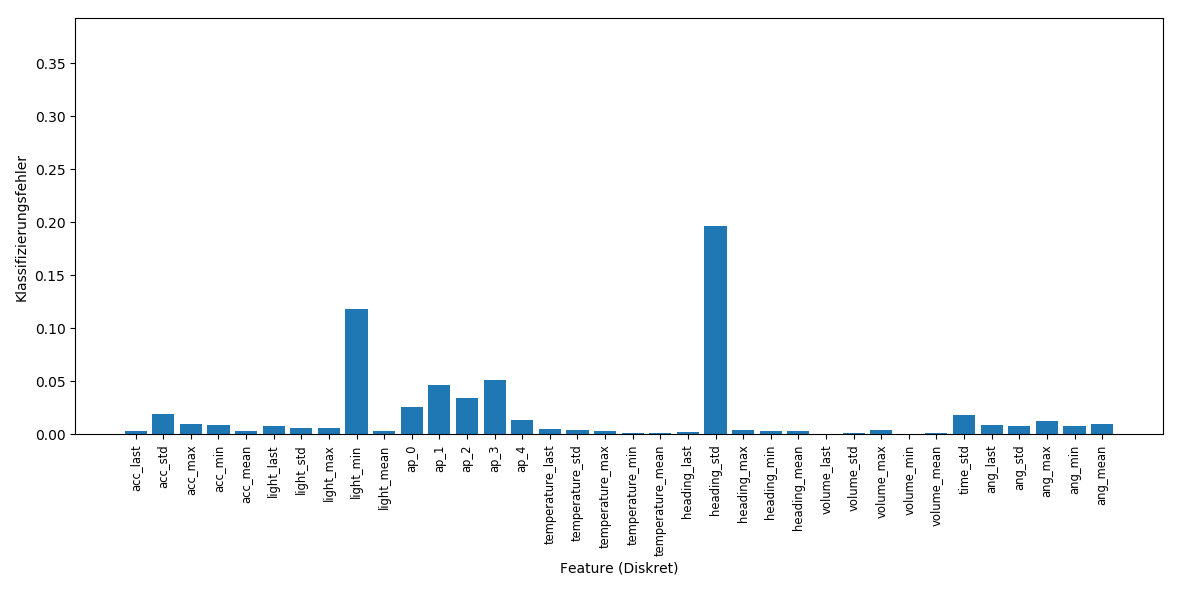
\includegraphics[width=\linewidth]{images/fi_wo_fe_dt.png}
    \caption{Permutationswichtigkeit der Features eines Entscheidungswaldes ohne Rückwärtskante.}
    \label{fig:feature_significance_dt_wo_fe}
\end{figure}
\begin{figure}[h!]
    \centering
    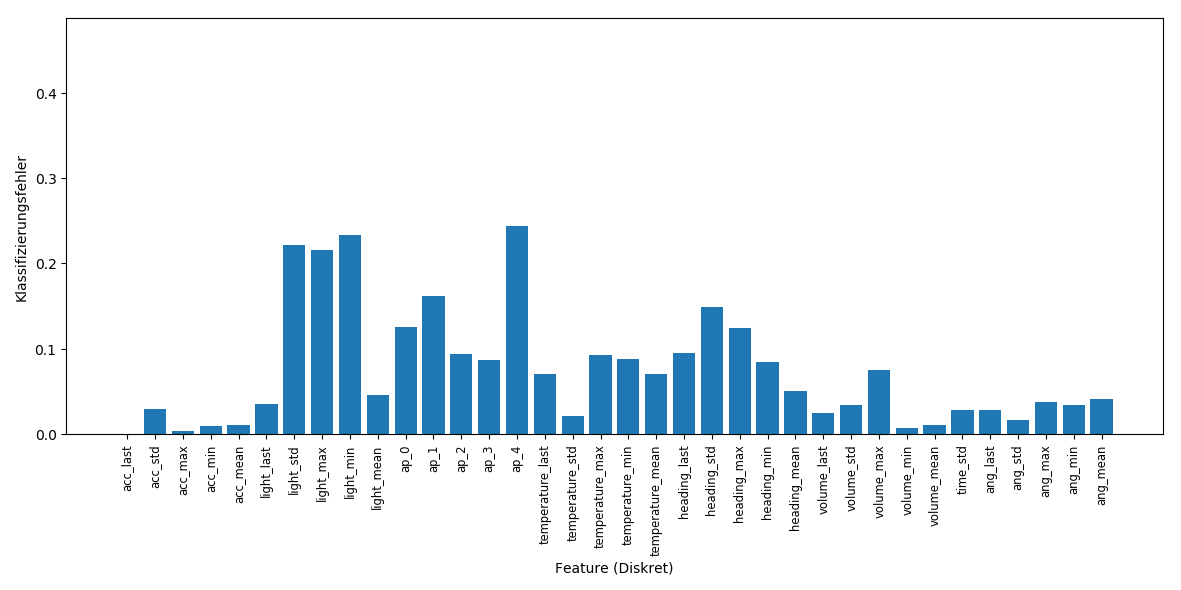
\includegraphics[width=\linewidth]{images/fi_wo_fe_knn.png}
    \caption{Permutationswichtigkeit der Features eines FFNN ohne Rückwärtskante.}
    \label{fig:feature_significance_knn_wo_fe}
\end{figure}
\newpage
Abbildung \ref{fig:feature_significance_dt_anomaly} zeigt die Permutationswichtigkeit von einem Entscheidungswald zur Anomalieerkennung.
Am wichtigsten sind die Features, welche die Wahrscheinlichkeitsverteilung des Klassifizierungsergebnisses von dem ML-Modell zur Standorterkennung ausnutzen.
Die Abweichung zu den durchschnittlichen Standortänderungen hat kaum Einfluss.
Dies deutet darauf hin, dass die ML-Modelle zur Standorterkennung nicht so instabil in Anomalien sind, wie angenommen.
Aus dem selben Grund hat das Feature der Topologieverletzung auch wenig Einfluss, da es bei Anomalien wenig ausschlägt.
\begin{figure}[h!]
    \centering
    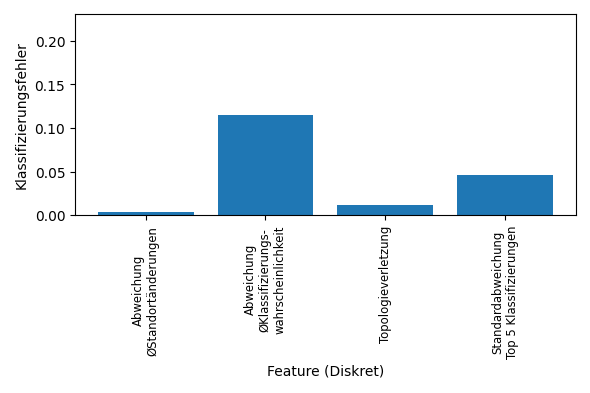
\includegraphics[width=0.65\linewidth]{images/fi_anomaly_dt.png}
    \caption{Permutationswichtigkeit der Features eines Entscheidungswaldes zur Anomalieerkennung.}
    \label{fig:feature_significance_dt_anomaly}
\end{figure}
\newpage
Die Wichitgkeit der Features variiert mit dem Szenario, indem die ML-Modelle eingesetzt werden.
Aus diesem Grund sollte die Analyse der Wichtigkeit der Features individuell für jedes Einsatzszenario durchgeführt werden,
womit durch eine sorgfältige Feature-Selektion die Klassifizierungsgenauigkeit und der Ressourcenverbrauch maximiert werden kann.